
\begin{figure}
	\centering
	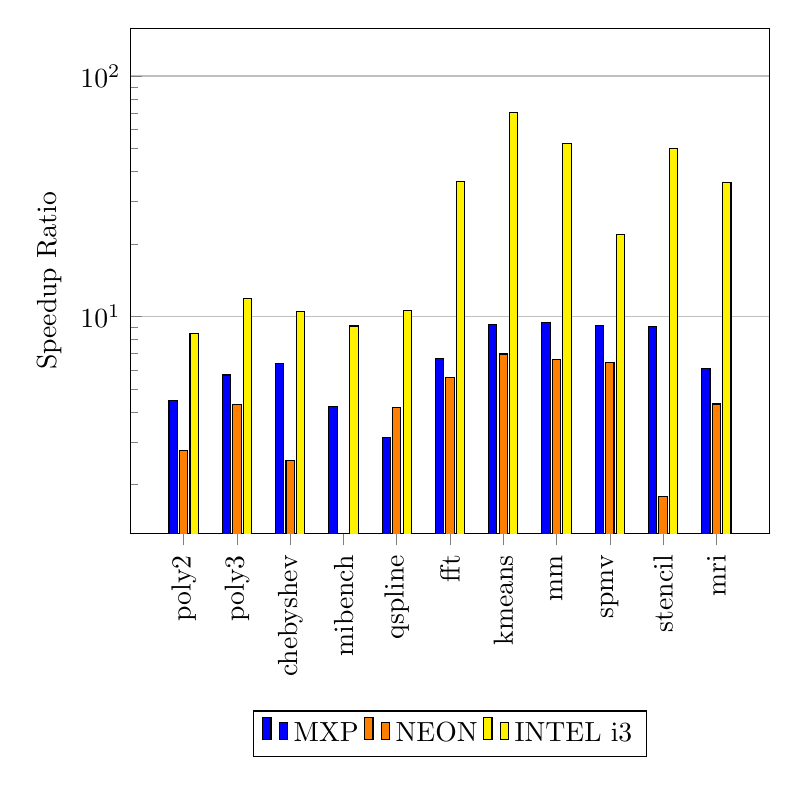
\begin{tikzpicture}
	\begin{semilogyaxis}[
	width  = 0.8*\textwidth,
	height = 8cm,
	xtick pos=left,
	ytick pos=left,
	%	major x tick style = transparent,
	x tick label style={rotate=90, anchor=east, align=right,text width=2cm},
	bar width=3pt,
	ymajorgrids = true,
	ylabel = {Speedup Ratio},
	symbolic x coords={poly2,poly3,chebyshev,mibench,qspline,fft,kmeans,mm,spmv,stencil,mri},
	xtick = data,
%	nodes near coords,
%	ybar,
%	every node near coord/.append style={rotate=90, anchor=west,font=\tiny, xshift=0.25cm},
	%	nodes near coords,
	%	ybar,
	%	every node near coord/.append style={rotate=90, anchor=west,font=\scriptsize},
	scaled y ticks = false,
	enlarge y limits={upper,value=0.2},
	%test
	%	enlarge x limits=0.25,
	ybar=2*\pgflinewidth,
	legend cell align=left,
	legend style={
		at={(.5,-0.35)},
		anchor=north,
		legend columns=-1
		column sep=0.5ex
	}
	]
	\addplot[draw=black,fill=blue]
	coordinates {(poly2,4.49) (poly3,5.709) (chebyshev,6.386) (mibench,4.22) (qspline,3.13) (fft,6.71) (kmeans,9.26) (mm,9.400) (spmv,9.1737) (stencil,9.0538) (mri,6.059) };
	
	\addplot[draw=black,fill=orange]
	coordinates	{(poly2,2.775 ) (poly3,4.32) (chebyshev,2.51) (mibench,1.25) (qspline,4.17) (fft,5.597) (kmeans,6.983) (mm,6.641) (spmv,6.4098) (stencil,1.784) (mri,4.326) };
	
	\addplot[draw=black,fill=yellow]
	coordinates	{(poly2,8.469 ) (poly3,11.834) (chebyshev,10.47) (mibench,9.122) (qspline,10.57) (fft,36.55) (kmeans,70.54) (mm,52.39) (spmv,21.96) (stencil,50) (mri,36.098) };
	
	\legend{MXP,NEON,INTEL i3}
	\end{semilogyaxis}	
	\end{tikzpicture}
	\caption{Byte level Speedup Analysis w.r.t ARMv7 for  different benchmarks.}
	\label{speedup:1}
\end{figure}
